\chapter{Building a Model of the System}
In the previous chapter, we have covered, how one calibrates and extracts the parameters necessary to model a qubit-resonator system under readout. We are now in a position to model it, however, with both many different levels of complexity and different available approximations at hand, we have a trade-off between run time of our simulations and the realism of them. 

\section{Different Simulation Approaches}
Thoughout the first few chapter, we covered different ways of representing and numerically integrating a quantum system. In this chapter, we will summarize the few methods. Some of the properties are summed up in table \ref{tab:simulation_types}

\begin{margintable}
    \caption{Caption}
    \centering
    \begin{tabular}{c|c|c|c|c}
                    &  SE   & ME    & MC    & SME \\ \hline 
    deterministic   & x     & x     &       &      \\
    dissipation     &       & x     & x     & x    \\ 
    backaction      &       &       &       & x    \\
    state size      & $n$   & $n^2$ & $n$   & $n^2$
    \end{tabular}
    \label{tab:simulation_types}
\end{margintable}

\begin{itemize}
    \item \textbf{Unitary} - This is a time evolution of the Schoedinger Equation \ref{sec: Time Evolution}. In Qutip this is done by the Adams algorithm which we covered in section \ref{sec:adams}. This is the fastest and simplest to run, but does not support interaction with the environment.  
    \item \textbf{Lindblad Equation} - The Lindblad equation simulates the density matrix and allows us to include dissipation terms. Like the Schoedinger equation, the Lindblad Master Equation is also deterministic, so it is only necessary to run it once for each configuration. All dynamics can then be extracted from $\rho$. 
    \item \textbf{Monte Carlo} - The Monte Carlo method is described in sec \ref{sec:monte_carlo} and the main idea is that the dissipations are applied stochastically and in between the dynamics are governed by the Schoedinger Equation. This allows for faster simulation than the Lindblad Master Equation. However, multiple trajectories will have to be taken to make sure the dynamics represent the full dynamics.
    \item \textbf{Stochastic Master Equation} - The Stochastic Master Equation is described in chapter \ref{sec:stochastic_master_equation} and the most complicated of the simulation tools. This includes the dynamics of the Lindblad Equation, but in addition also supports the weak measurement which is obtained during a readout.
\end{itemize}\todo{Citations}

\subsection{"Calibrating" the simulation}
To compare the different simulation methods, we repeat some of the calibration protocols from chapter \ref{chapter:calibrations}. Since the goal of this thesis is to model the readout, we are focusing on replicating the features relevant for readout. Since the Stochastic Master Equation is expensive to run, we will only use it, when the measurement records are necessary. We will thus test the Schoedinger Equation, Monte Carlo and Lindblad equation on some simple calibration schemes. 

The simulation are made by using the Hamiltonian for the full time-dependent Hamiltonian for the system given by equation \ref{eq:full_hamilton} and adding a contribution from a drive, where it is applicable. The parameters are taken from table \ref{tab:cali}made using $f_{01}$ ... from the cal

A collection of the simulation results from resonator spectroscopy, $T_1$ calibration and ... are found on page \pageref{fig:big_figure_test}. We note the following :

\begin{margintable}
    \centering
    \caption{Simulation Time Comparison for the figures seen in  ... }
    \begin{tabular}{c|c}
         &  \\
         & 
    \end{tabular}
    \label{tab:my_label}
\end{margintable}

In calibrating photon decay rate $\kappa$ and the temperature, we use more data from a single trace than just its average expectation value. Thus we will also include simulation in the Stochastic Master Equation.  \todo{Use MC as well? Don't need it, but need an argument} 

\todo{Comment on the figure and the results.}

% \begin{figure*}[h]
%     \centering
%     % \missingfigure{$T_1$ Calibration for the different simulations. }
%     % \label{fig:enter-label}
%     % \missingfigure{$T_2$ Calibration for the different simulations. }
%     \caption{Caption 2}
%     \label{fig:big_figure_test}
%     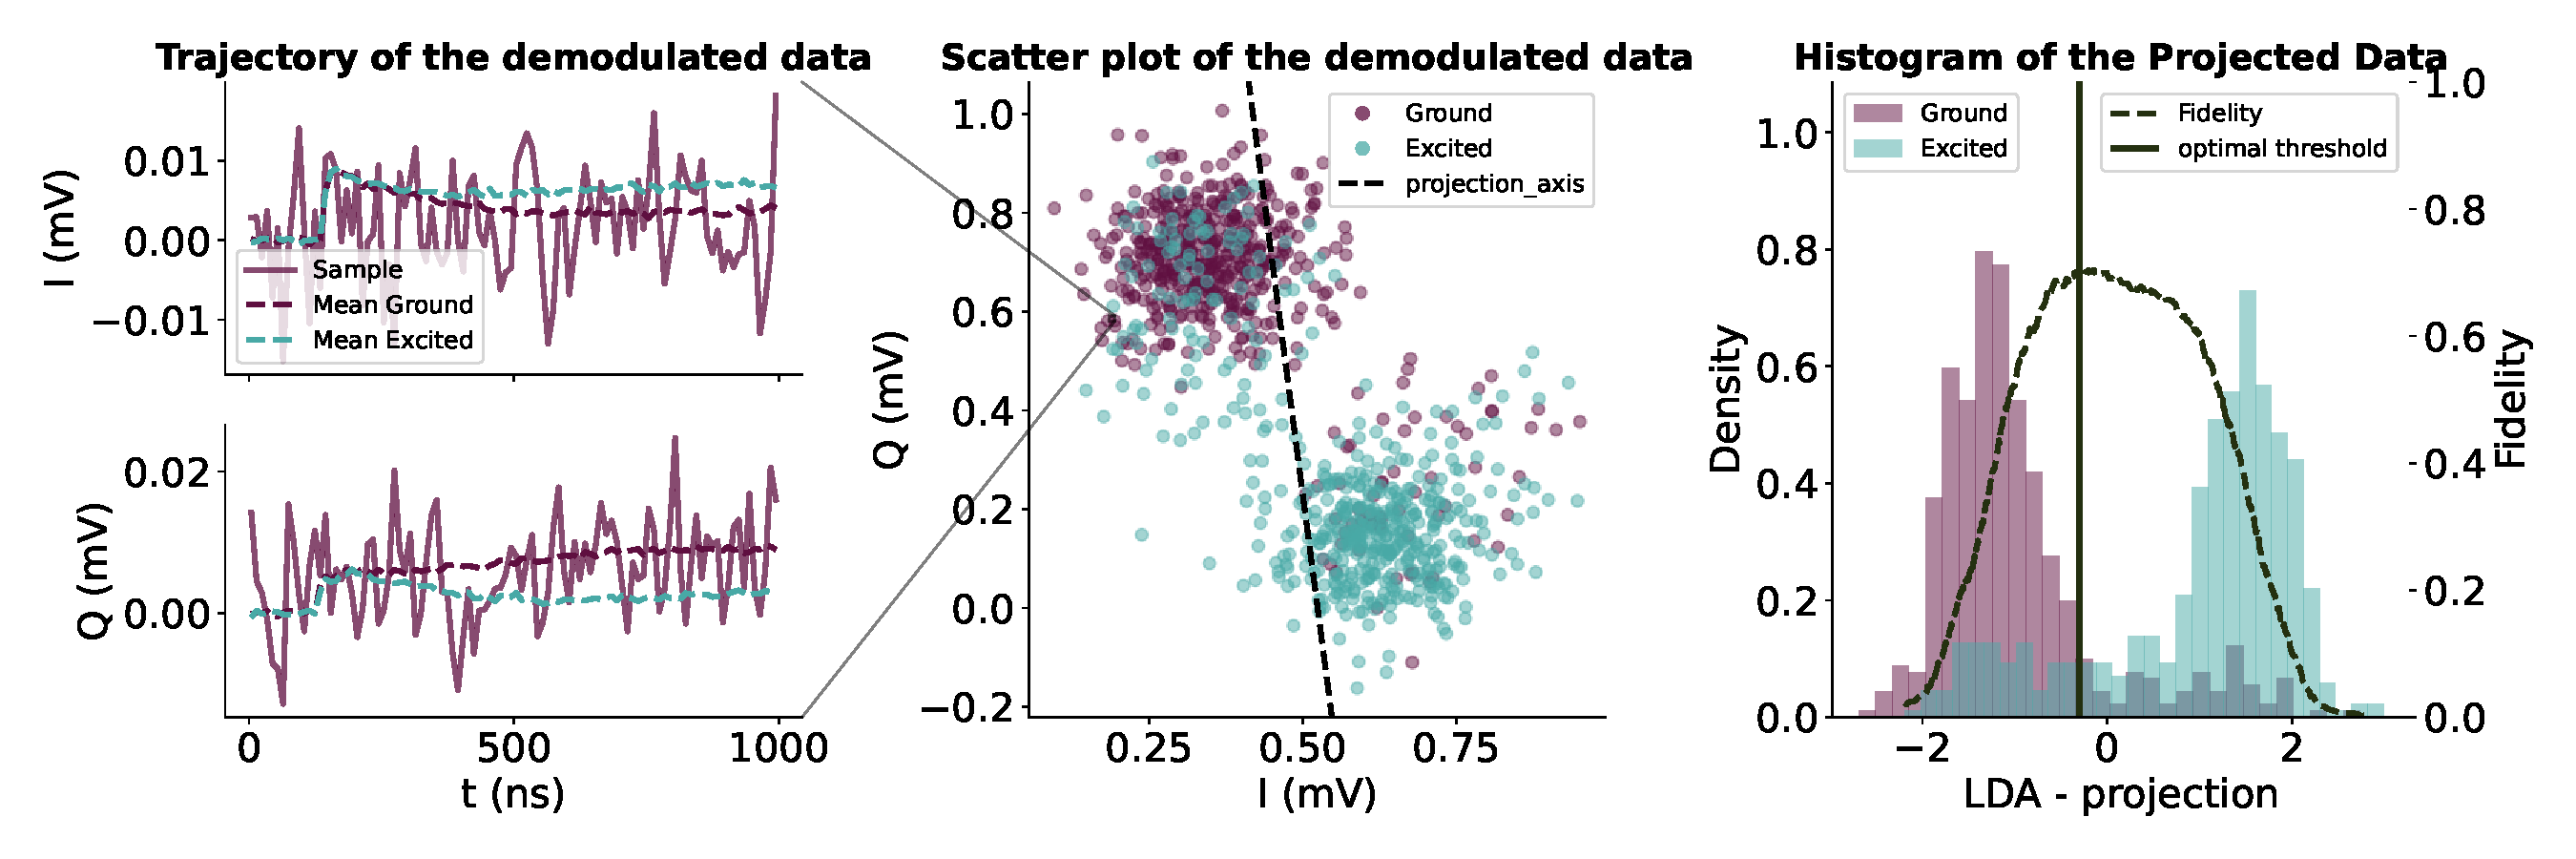
\includegraphics[]{Readout/Figs/Introduction.pdf}
%     \hspace{2 cm}
%     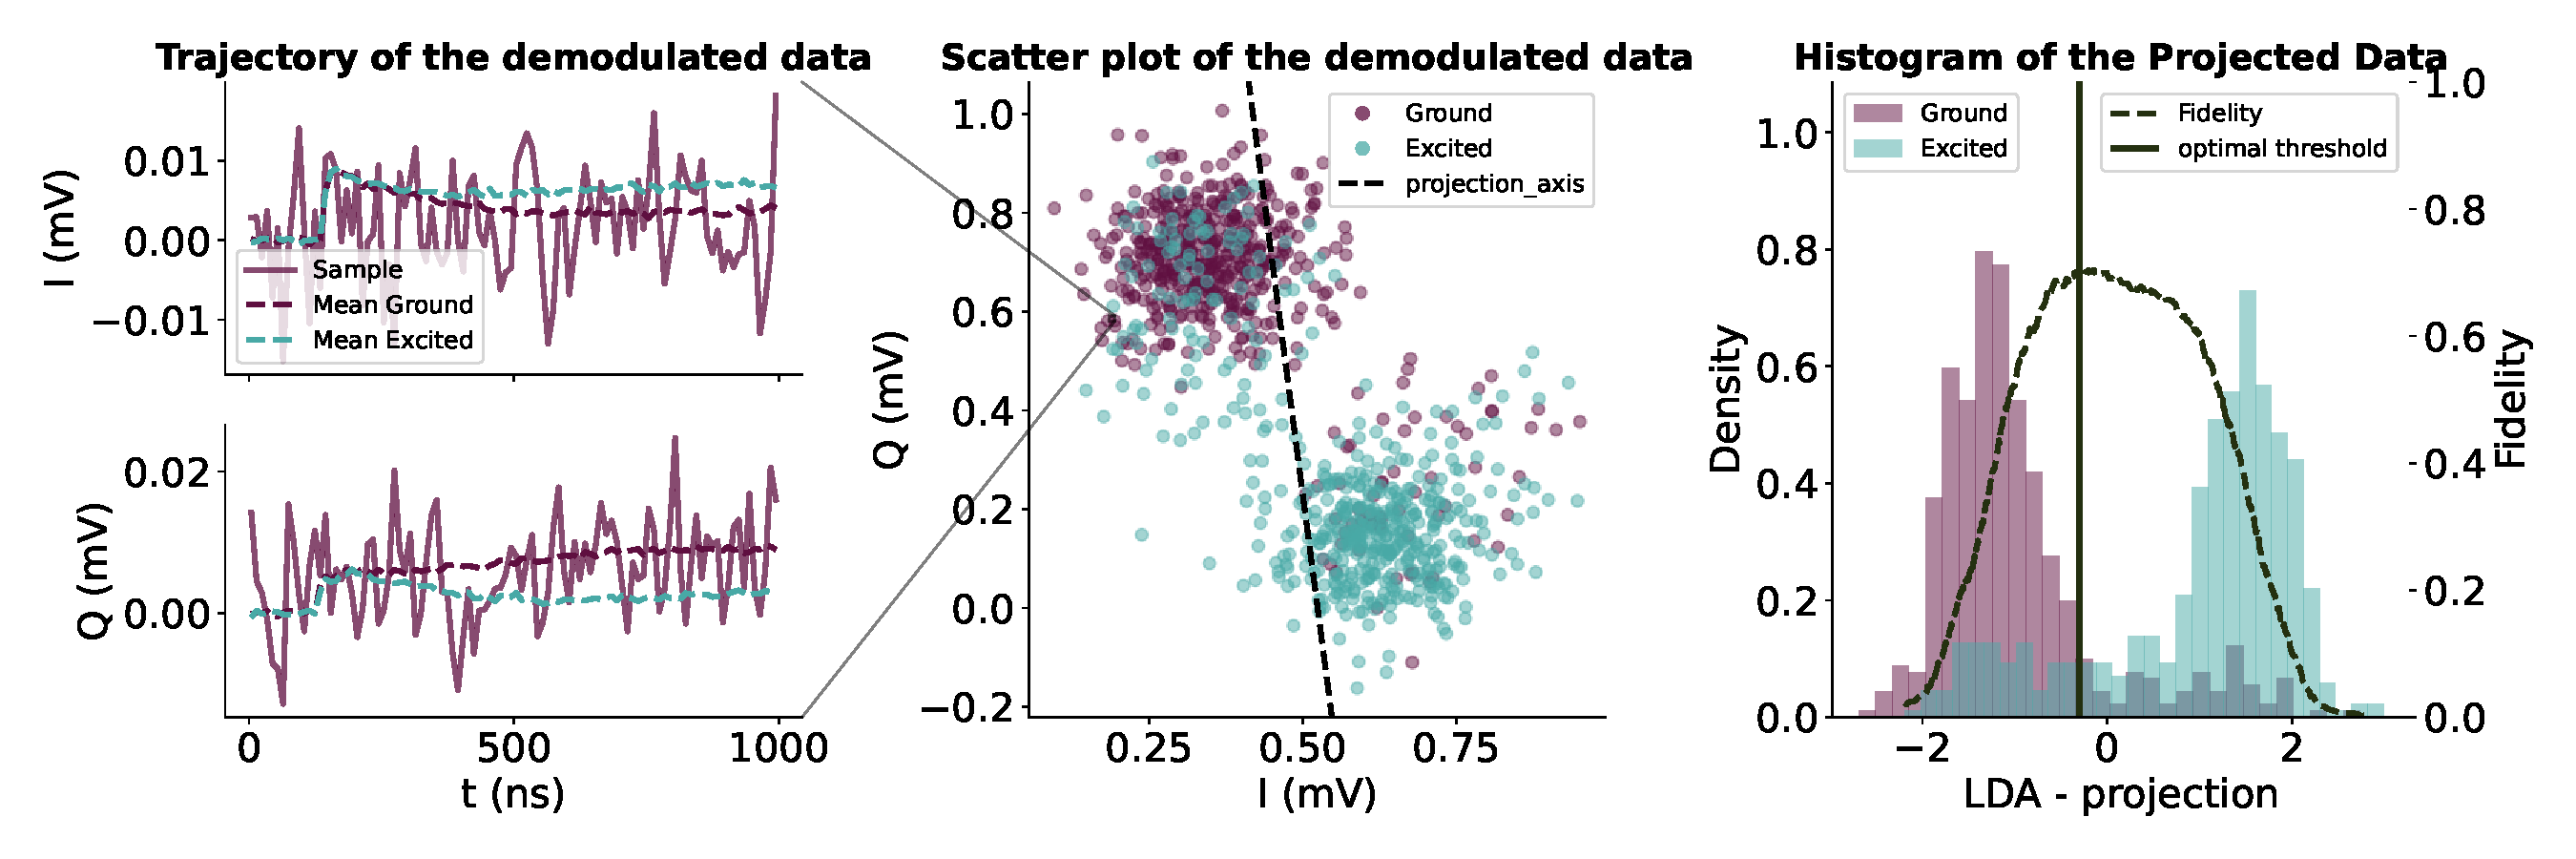
\includegraphics[]{Readout/Figs/Introduction.pdf}
%     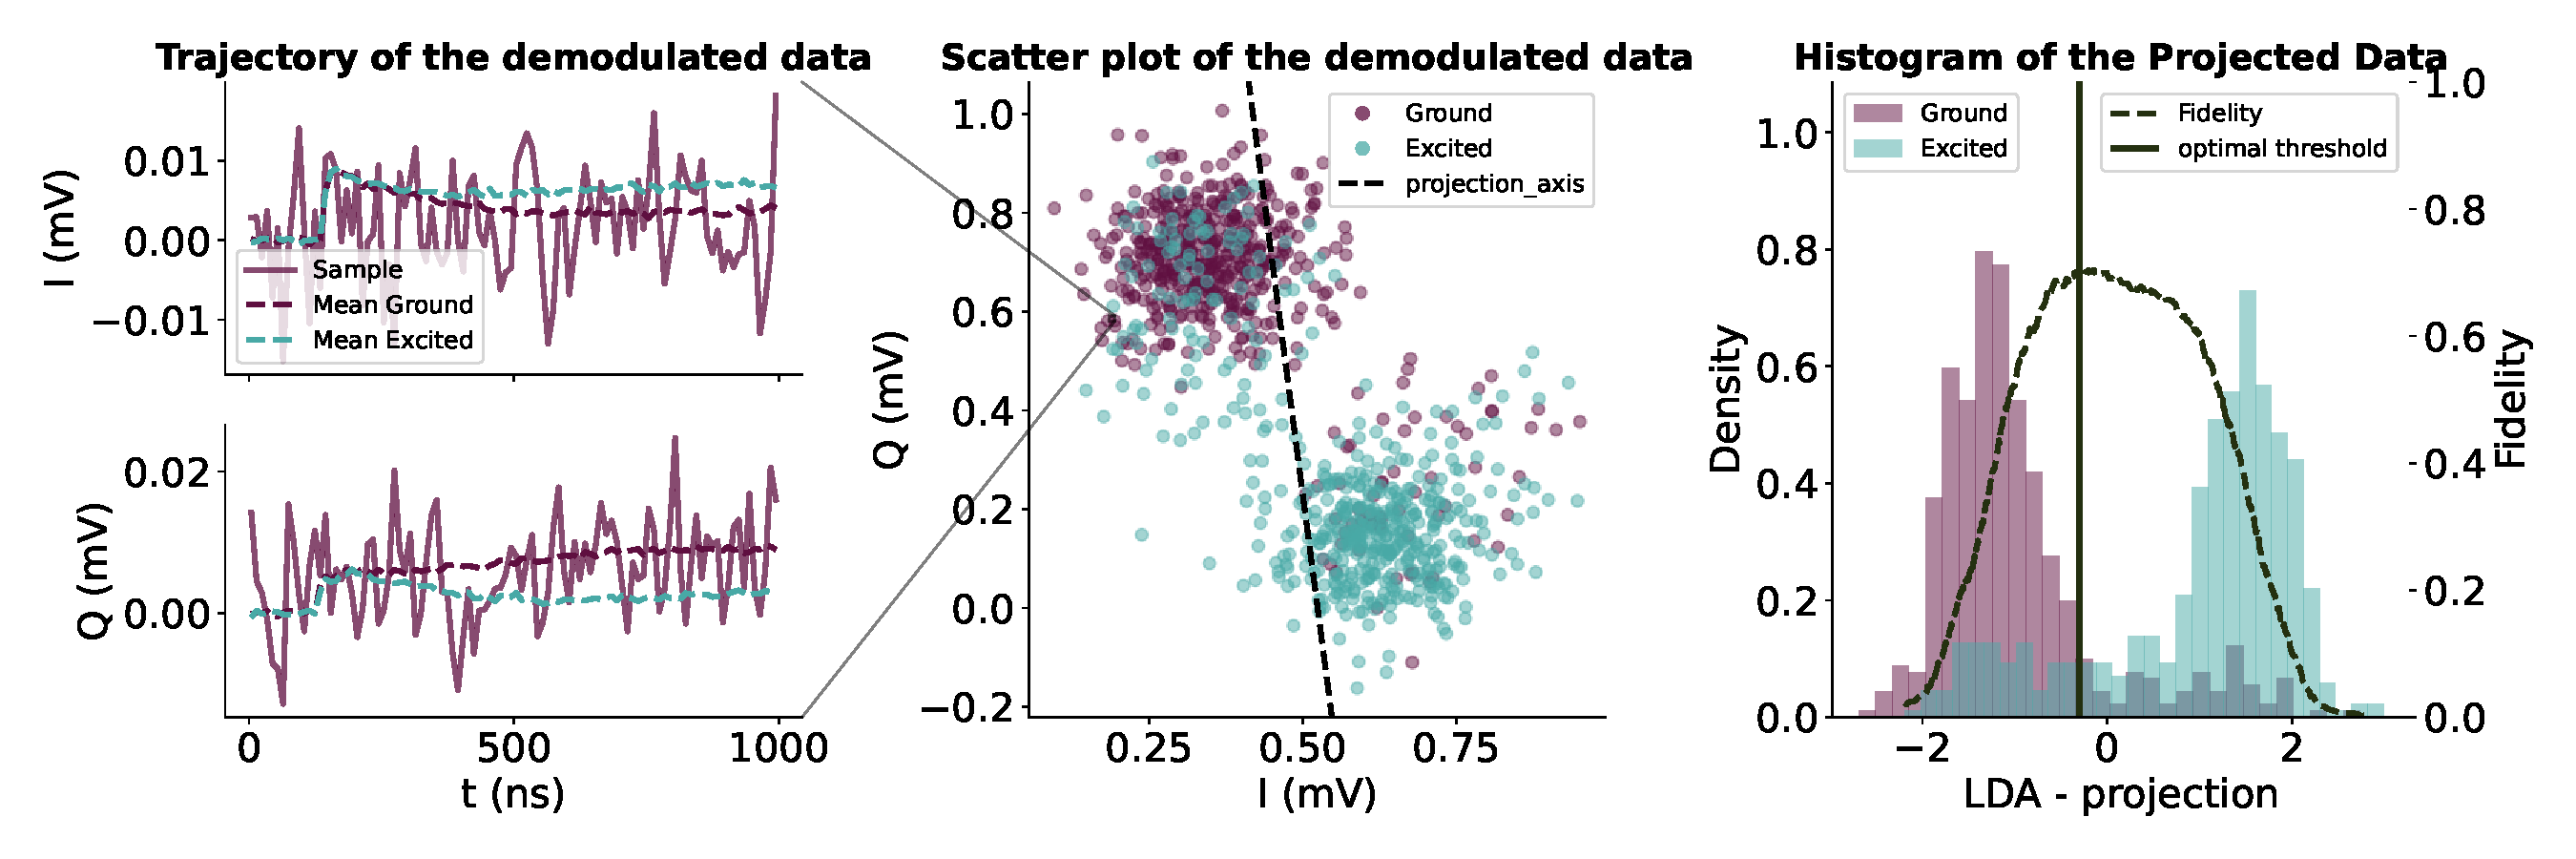
\includegraphics[]{Readout/Figs/Introduction.pdf}
%     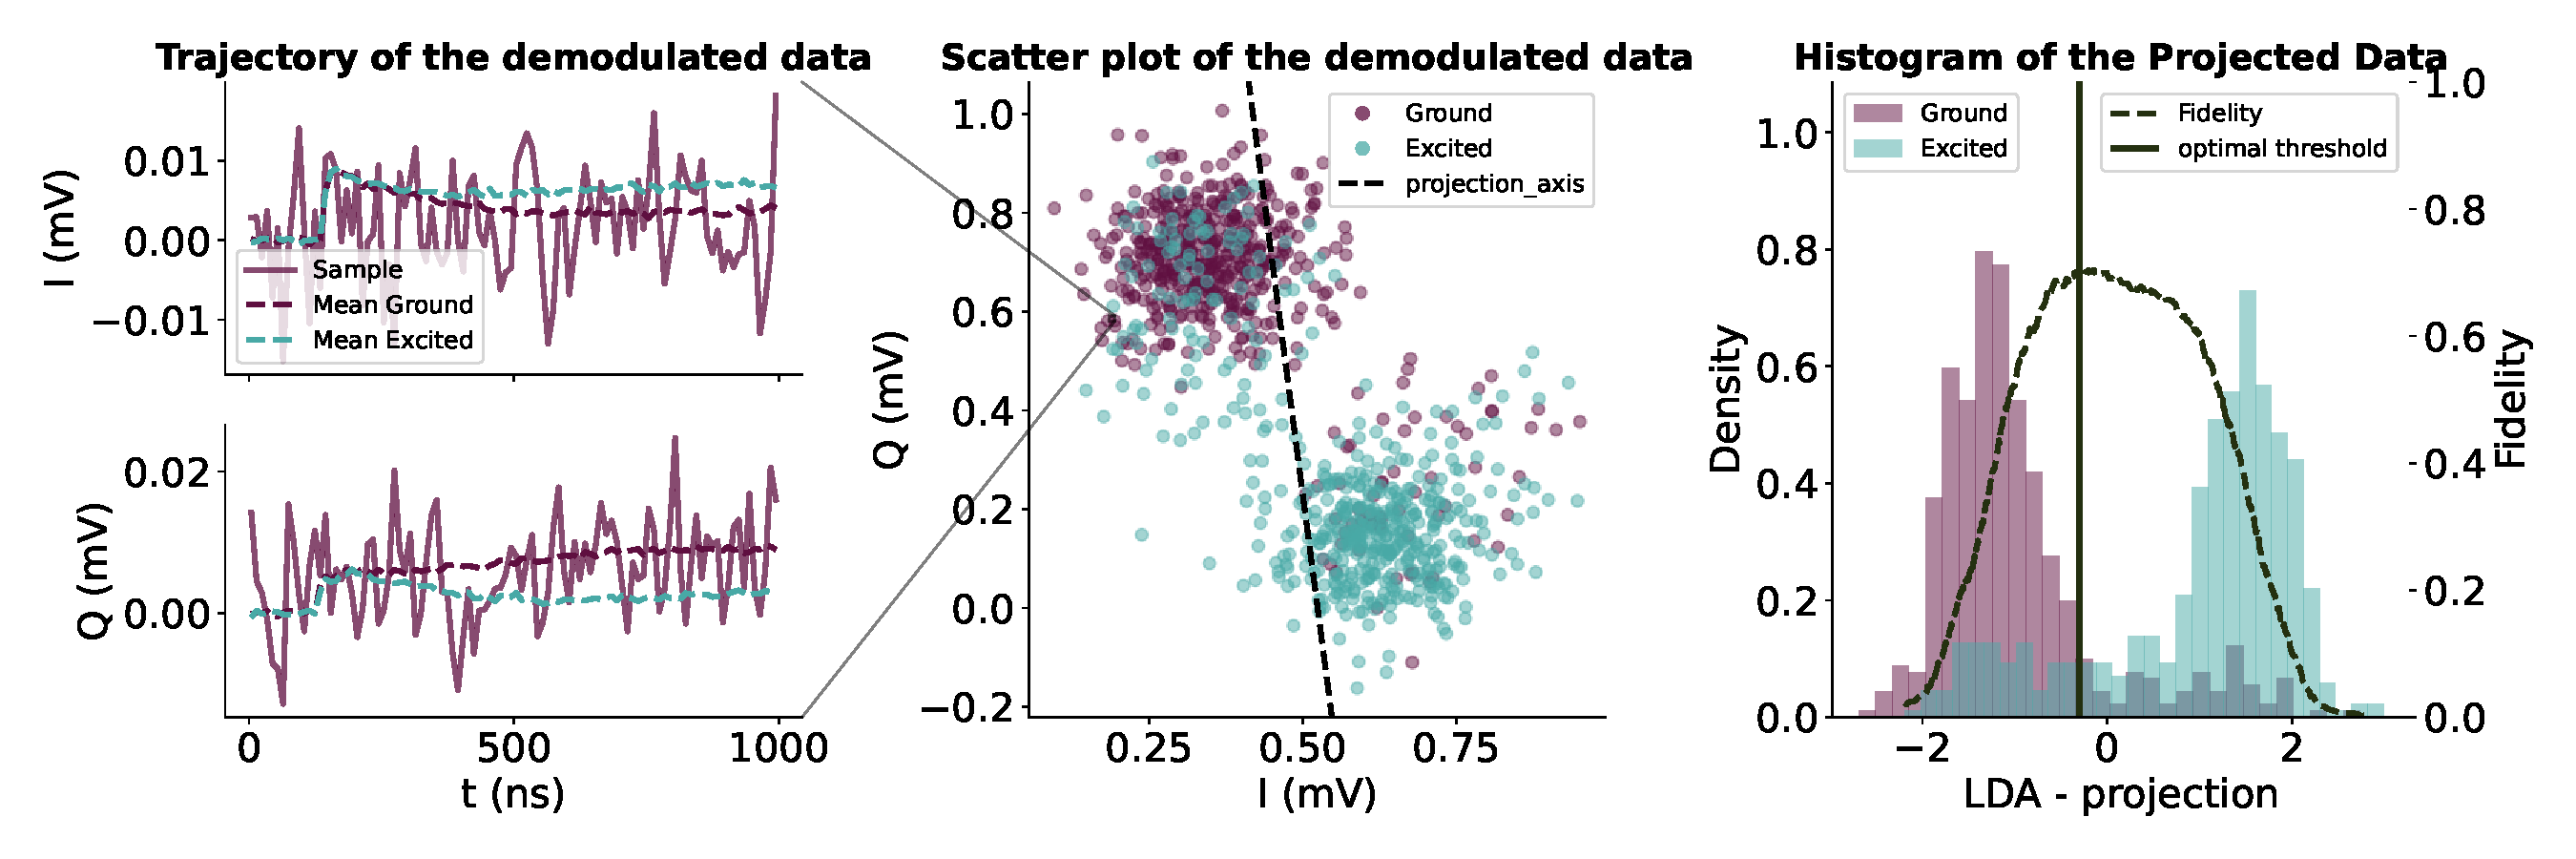
\includegraphics[]{Readout/Figs/Introduction.pdf}
% \end{figure*}

\begin{figure}[h]
    \begin{minipage}{0.45\textwidth}
        \centering
        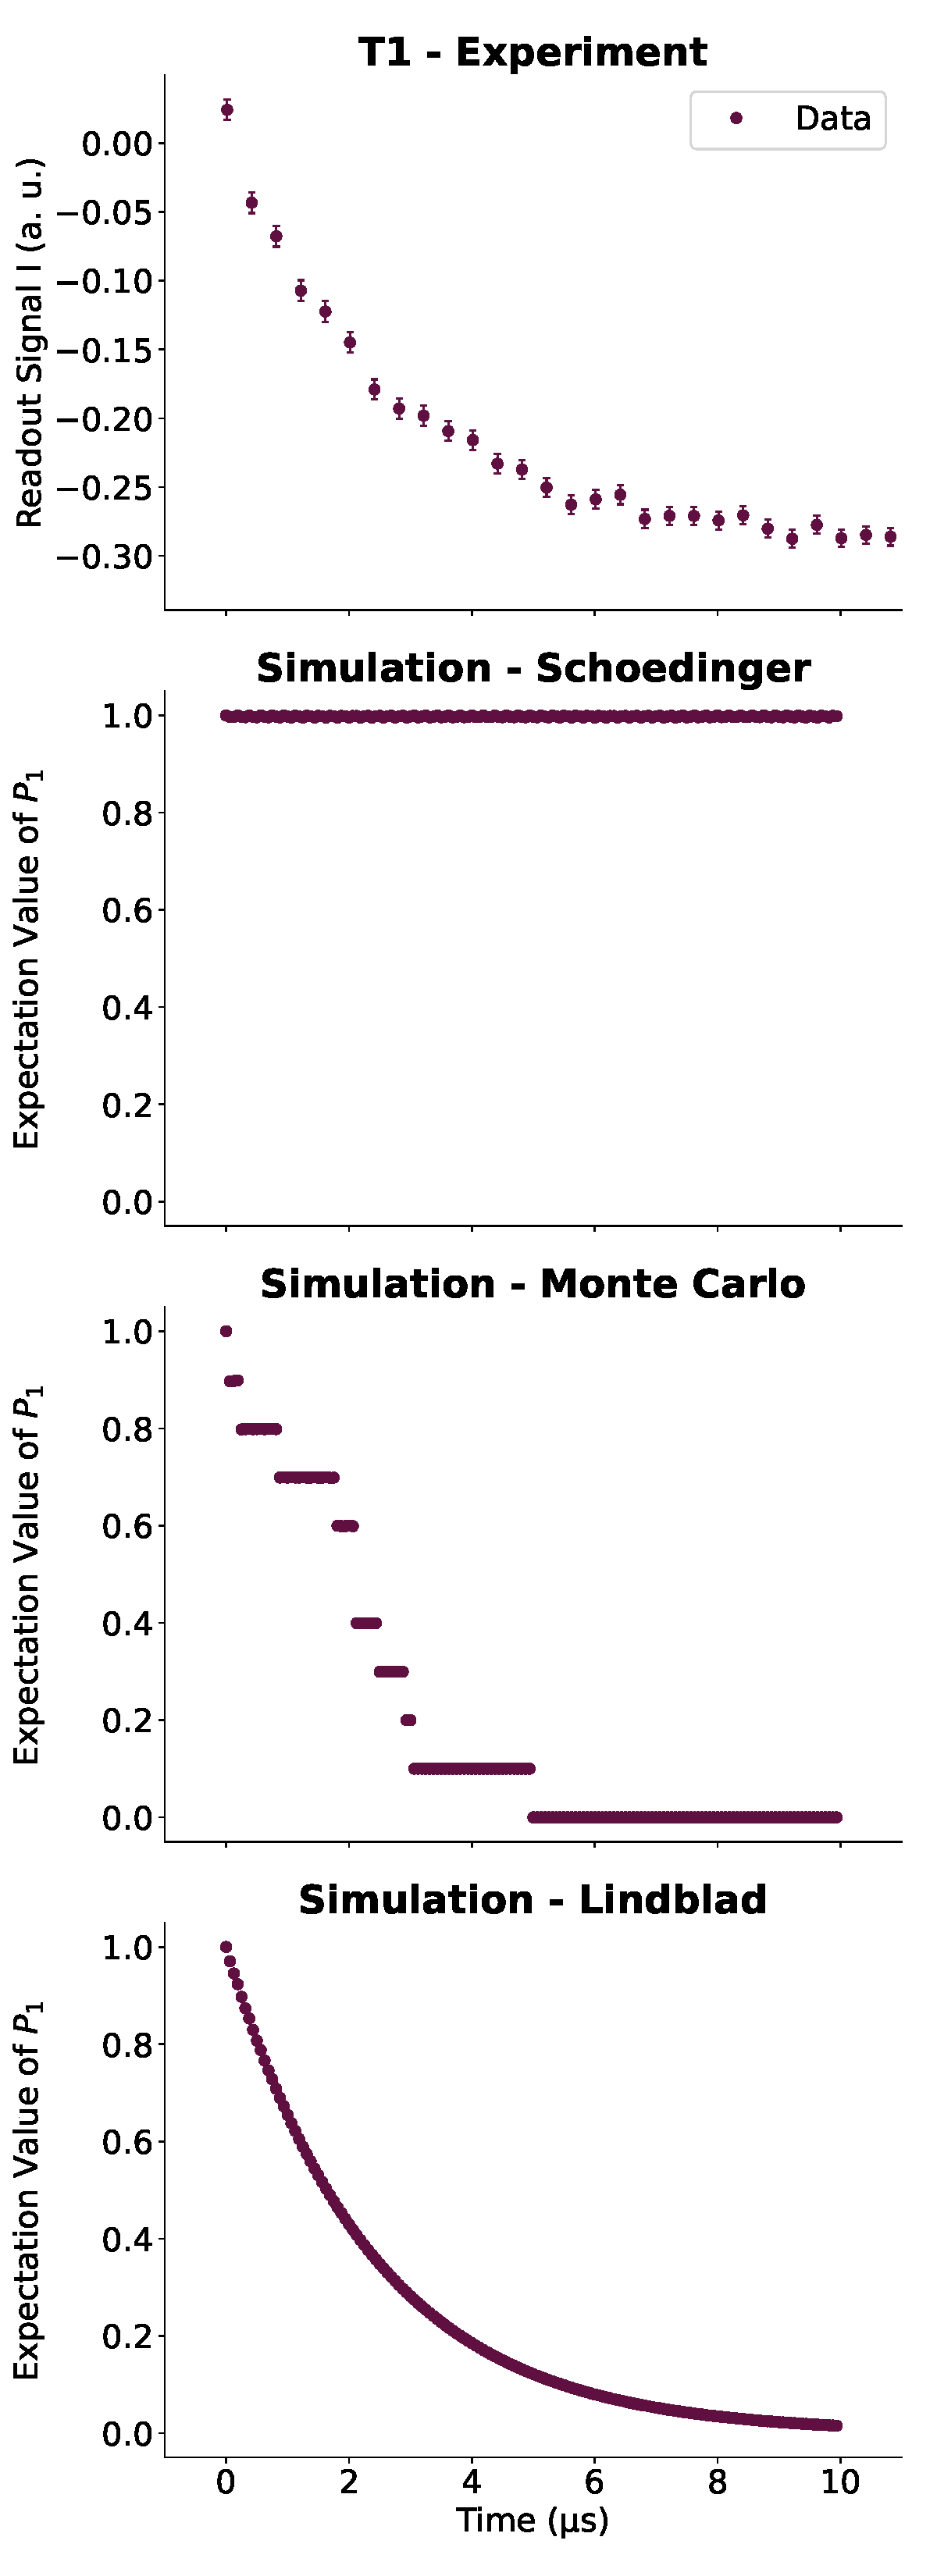
\includegraphics[]{Simulations/simulations_of_calibrations/Figs/qubit_T1.pdf}
    \end{minipage}
        \begin{minipage}{0.45\textwidth}
        \centering
        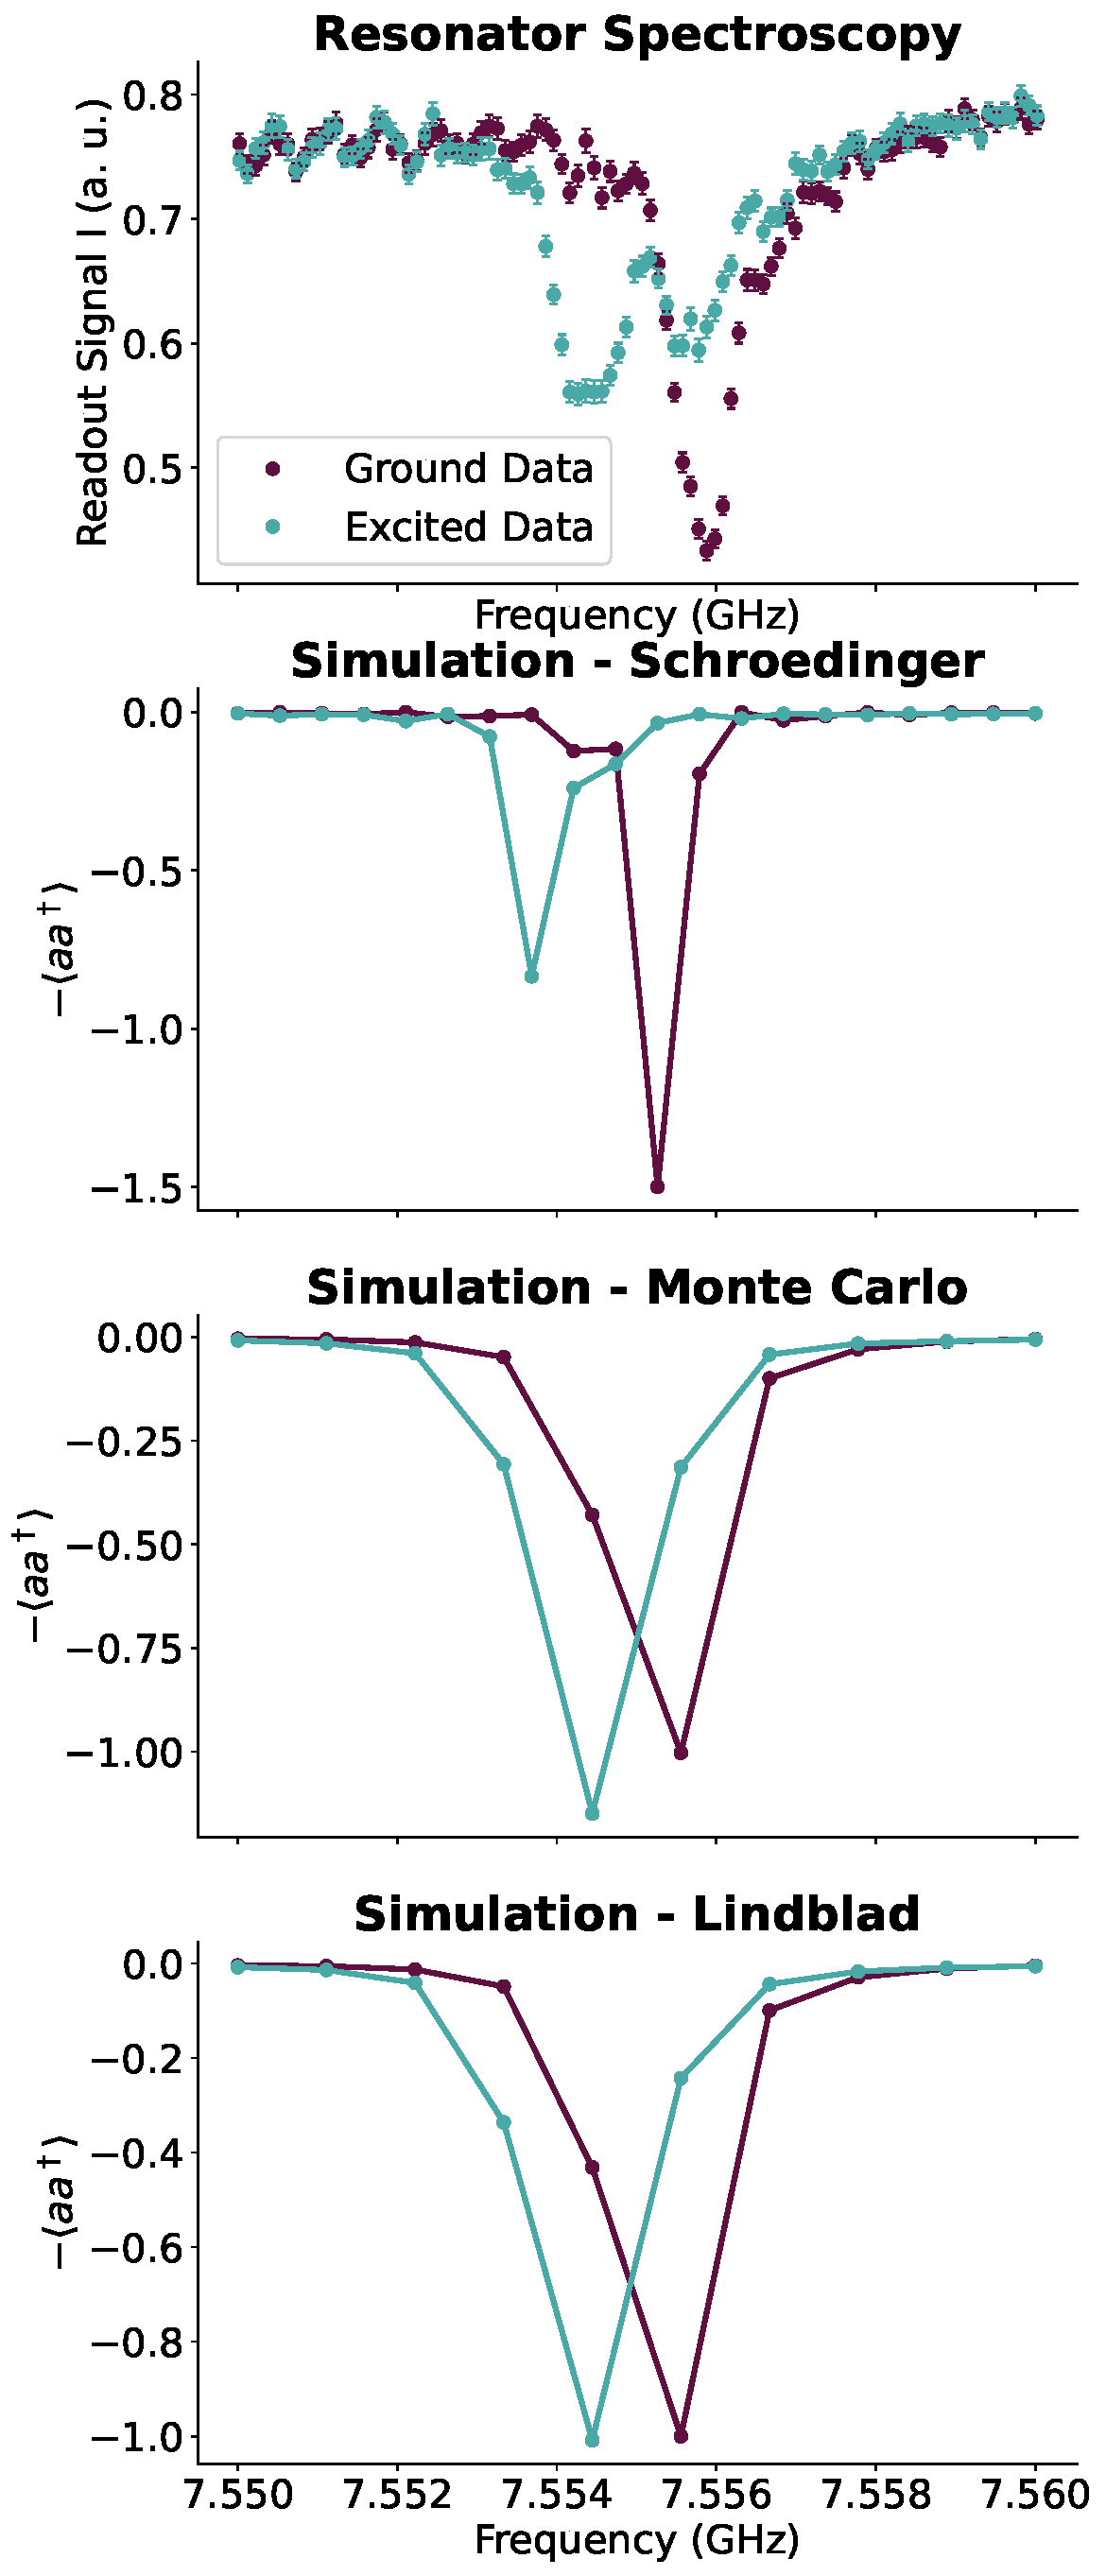
\includegraphics[]{Simulations/simulations_of_calibrations/Figs/resonator_spectroscopy.pdf}
    \end{minipage}
    \caption{Illustration of the $T_1$ and resonator spectroscopy run with different simulations schemes.}
    \label{fig:calibrations_in_simulation}
\end{figure}



% \begin{figure}
%     \centering
%     \missingfigure{Calibration Scheme of $\kappa$ measurements}
%     \missingfigure{Calibration Scheme of $\tau$ IQ plot ? } 
%     \caption{Caption}
%     \label{fig:enter-label}
% \end{figure}

\FloatBarrier

\subsection{Q Function and Trajectories}
When we consider the Lindblad equation, the result is a deterministic list of density matrices at each point in time. This is also a possiblity, when we integrate the Stochastic Master Equation, but in addition, we have the simulated trajectories which resemble the contious weak readout done in the laboratory. In order to compare these two methods, we will make use of the Q-function represented in \ref{sec:QFunc} which illustrates a 2-dimensional probability density of the quadratures in the resonator. 

If we simulate the readout process of the qubit-resonator system under the dispersive approximation, we can compare the measurement records from the Stochastic Master Equation with the evolution of the Q-function from the Lindblad Equation. This is summarized in figure \ref{fig:trajectories_and_qfunc}

\begin{figure*}[h]
    \centering
    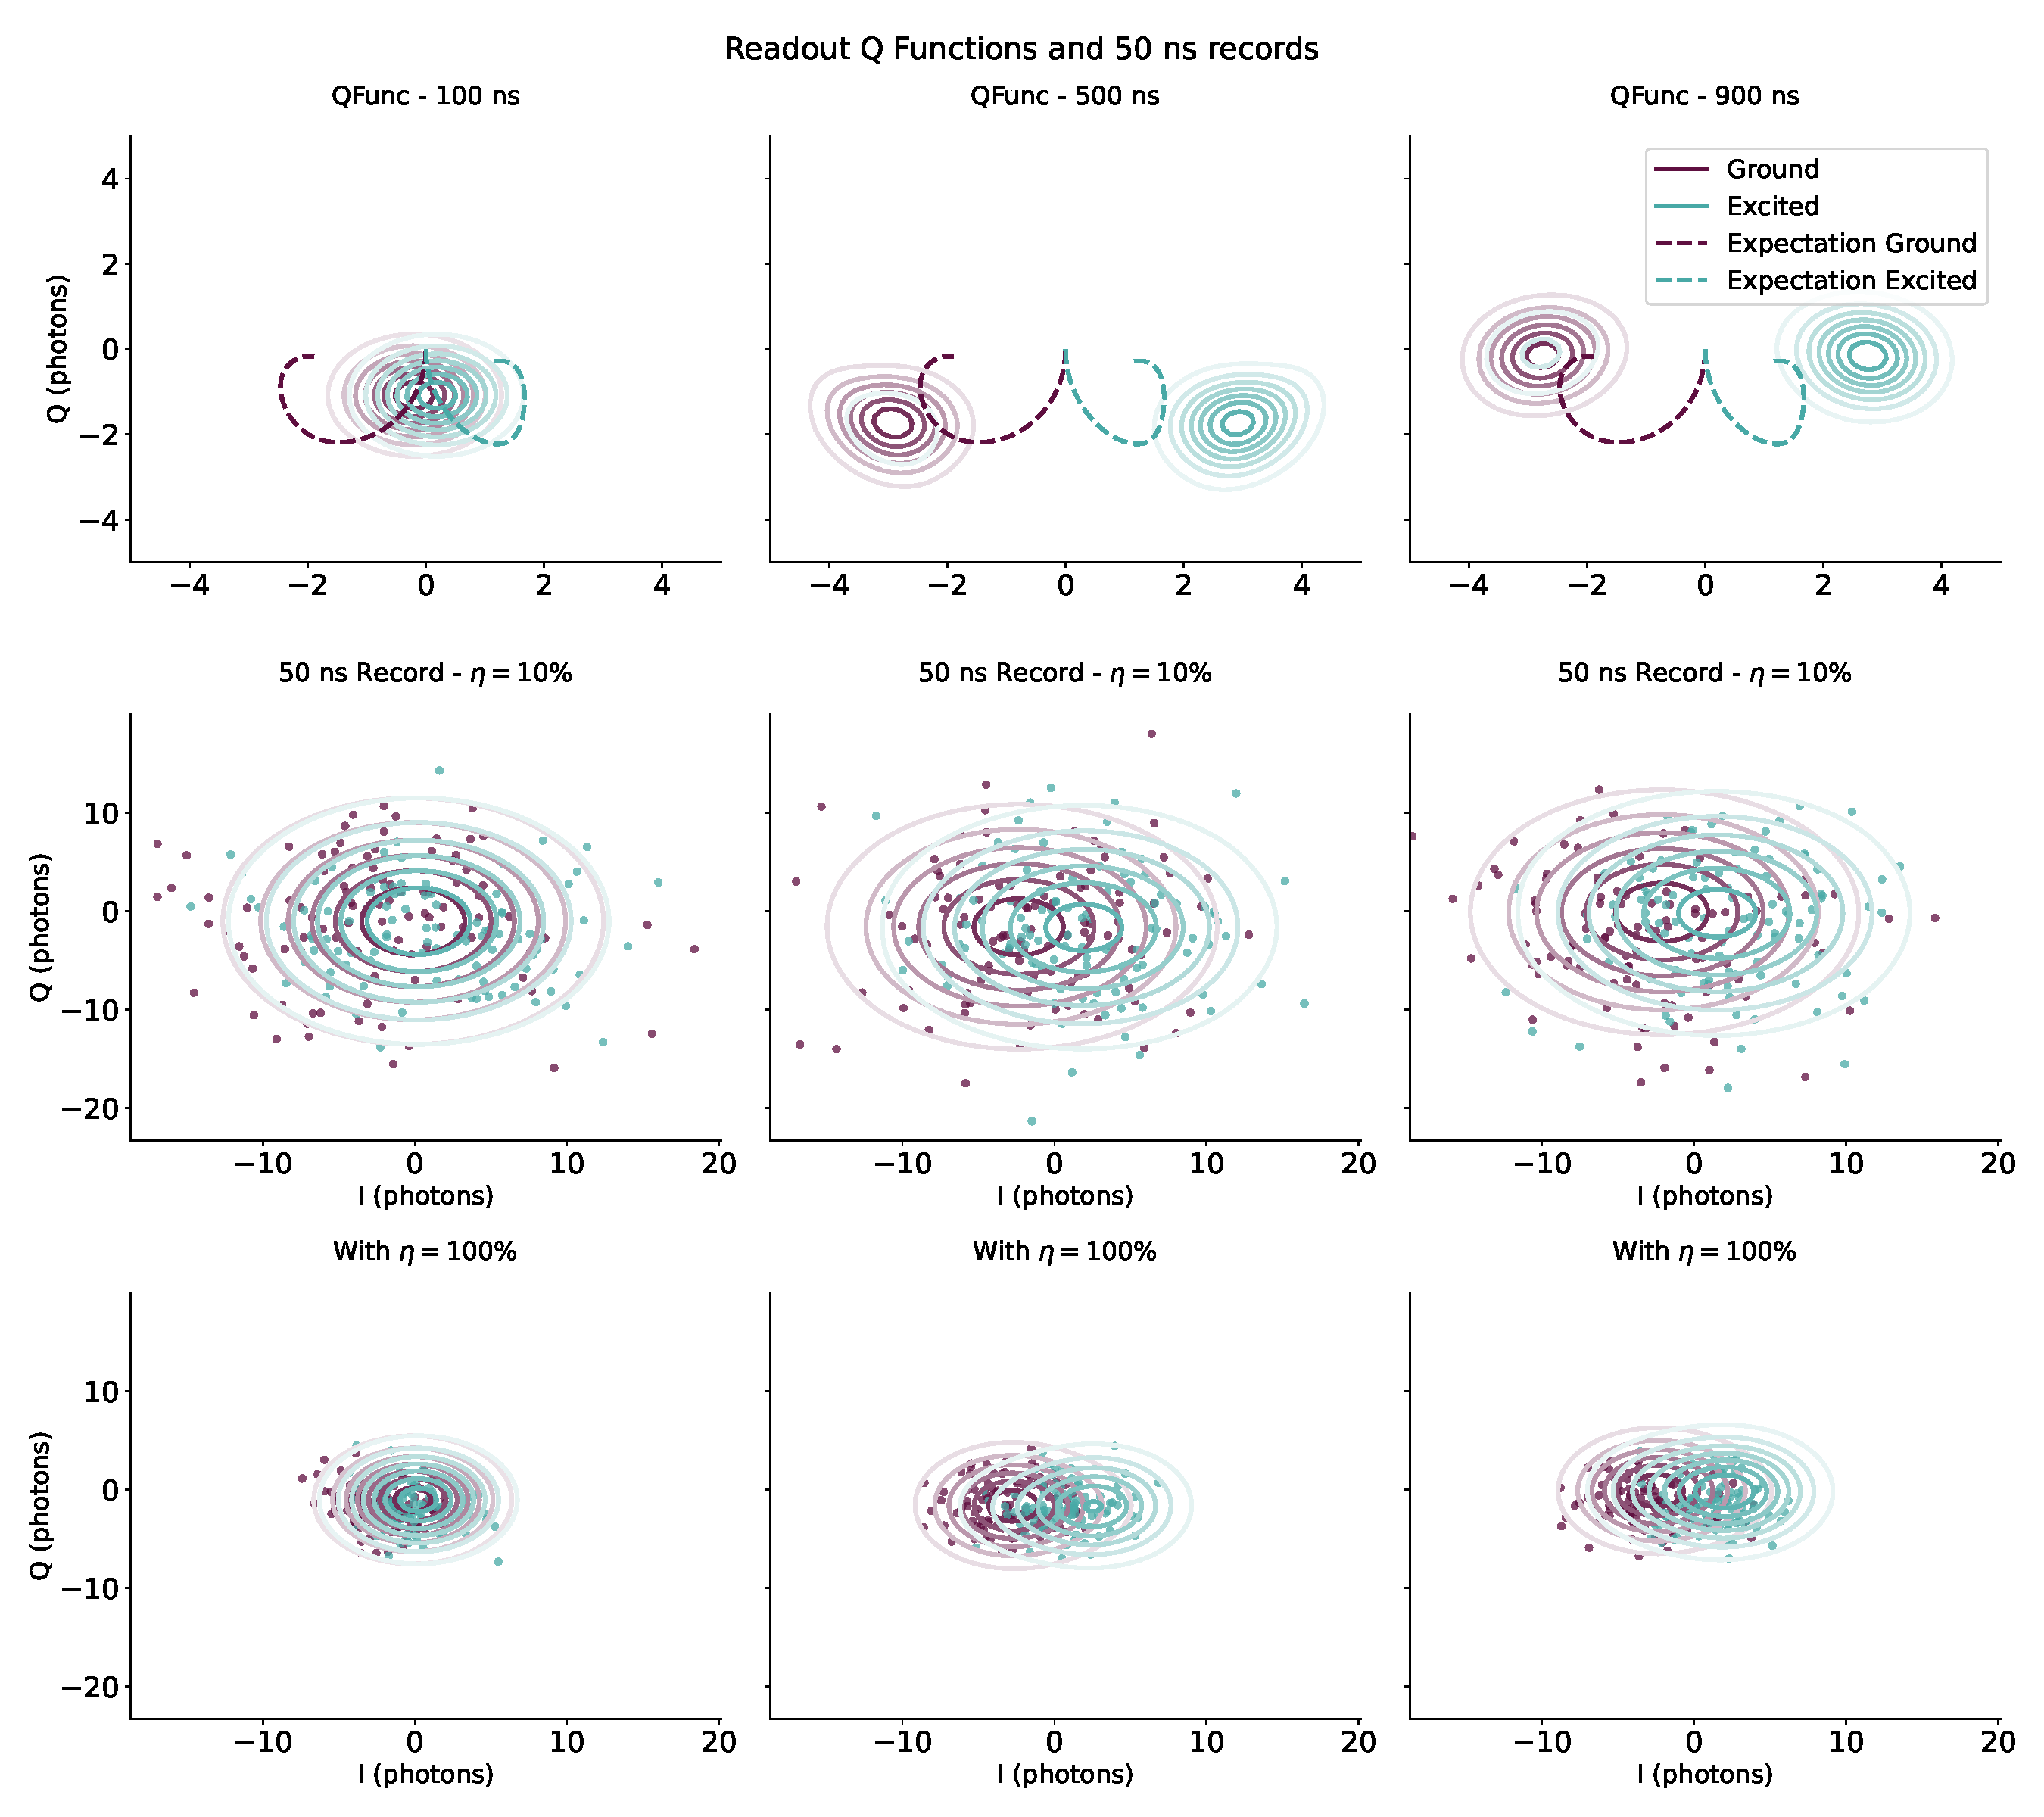
\includegraphics[]{Simulations/readout_simulations/figures/qfunc_trajectories.pdf}
    \caption{Comparison of the Q Function and the scatter plot for a 10 ns readout record. In the top plot the Q Function distribution is shown at $t = 0, 200$ and $400 \text{ ns}$. In the two lower rows the the measurement record for 250 $\ket{0}$ and $\ket{1}$ trajectories are shown. Furthermore, the Q-Function is convolved by a 2d Gaussian with covariance matrix $2 \Delta t / \eta \identity$ to match the error of the records.}
    \label{fig:trajectories_and_qfunc}
\end{figure*}

The measurement record is given by a term proportional to the expectation value of the measured quantity and a noise term, which in the derivation from chapter \ref{sec:} was a Gaussian. For a perfect coherent state, this is closely to the distribution of its Q function. Especially in the hetereodyne measurements. For a state, we can get a somewhat approximation. We need to scale the standard deviation with eta. Furthermore, we get a reductioon depending on the time of the measurement. This gives the good idea of measuring.... \todo{This is really just me writing sentences which could be included}





\section{Validity of the Dispersive Approximation}
The full time-dependent Hamiltonian, we simulated to get the results shown in figure \ref{fig:calibrations_in_simulation} are expensive to run. The largest part of this process is to calculate the time-dependent function of the pulse. In the dispersive approximation which we covered in section \ref{sec:dispersive} we could eliminate the time-dependence of the pulse by going to another basis.

Before continuing with the approximation, we will first test whether it still exhibits the behaviours, we need to investigate the readout. 

\begin{figure}
    \centering
    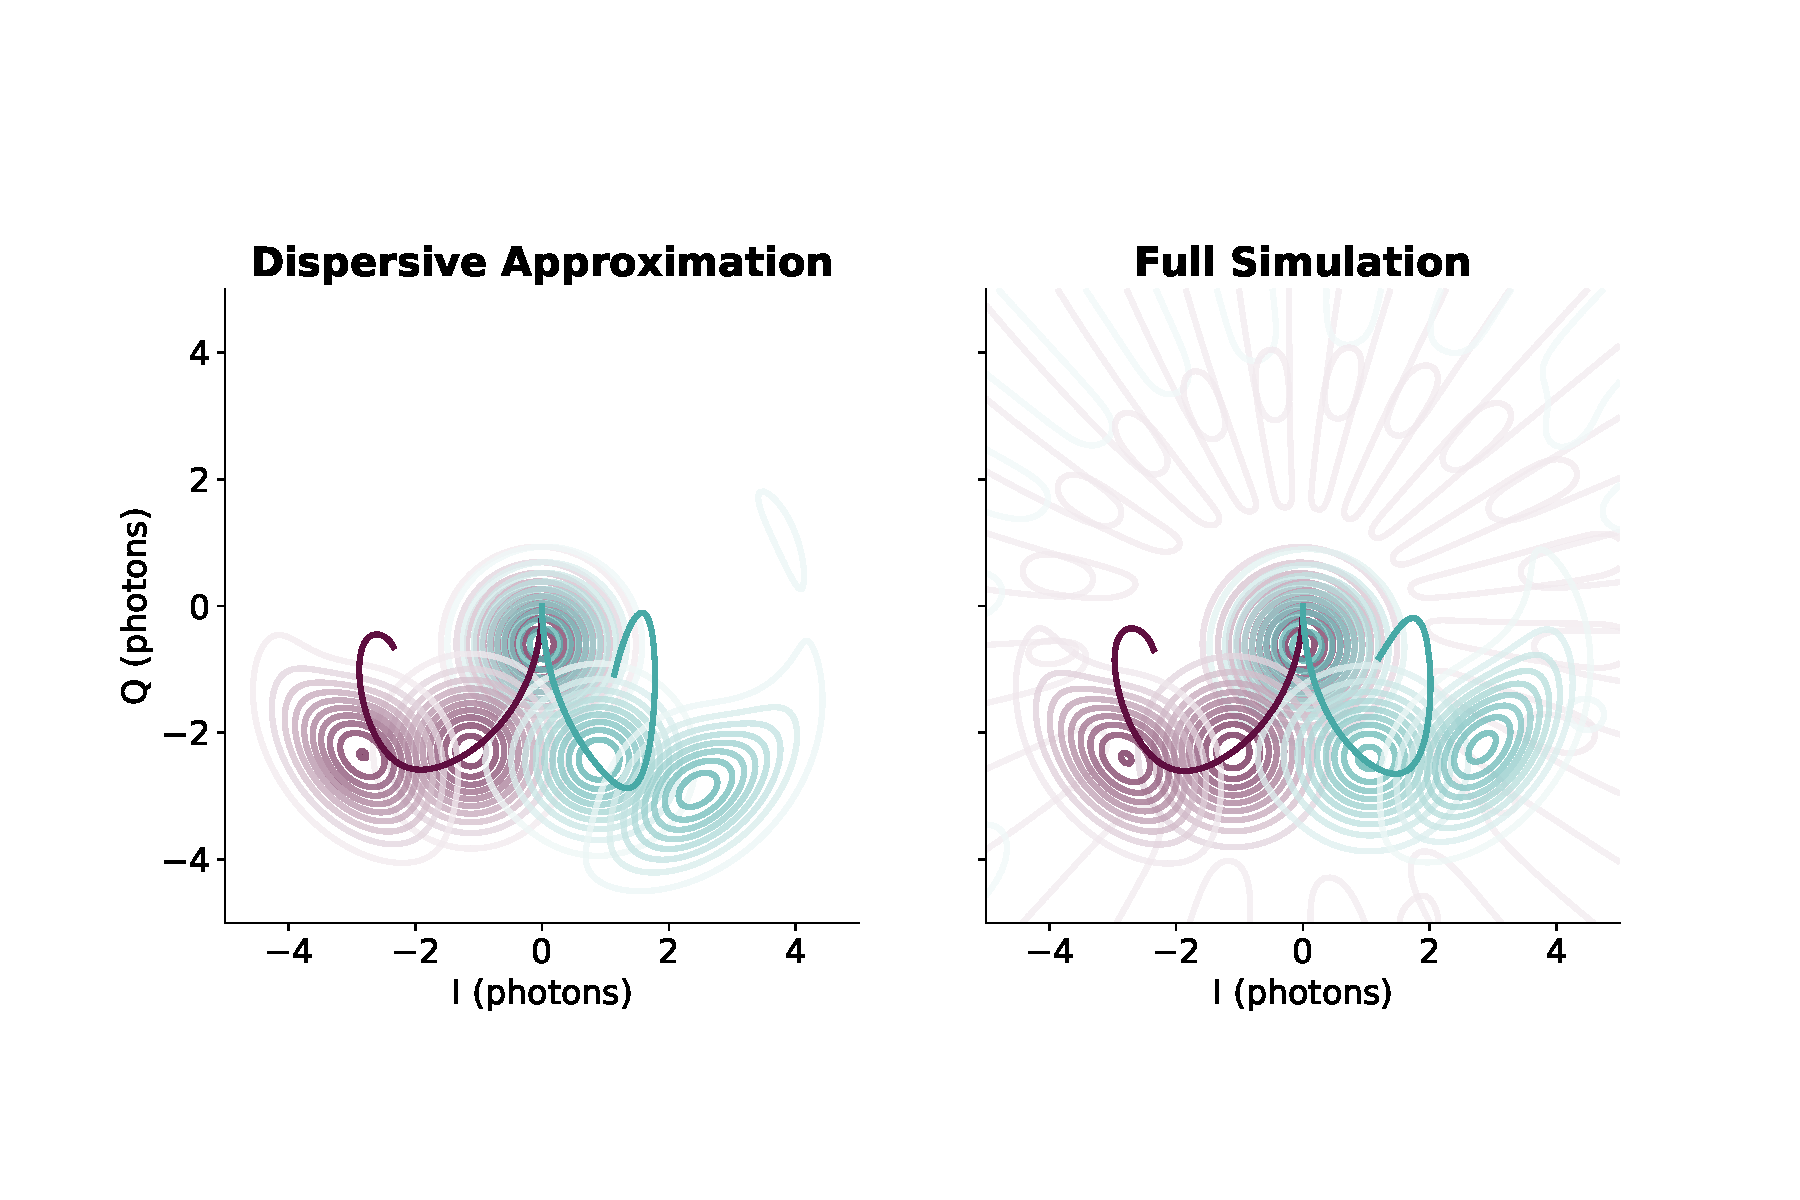
\includegraphics[width = \textwidth]{Simulations/readout_simulations/figures/dispersive_approx.pdf}
    \caption{Caption}
    \label{fig:enter-label}
\end{figure}

\subsection{The Punchout}
In the dispersive limit, we consider that $g/(\omega_r - \omega_q) \ll 1$, which has be sufficient for us since we consider low-photon-number readout. If we were to increase this to the high power regime, one starts to see a lot of interesting physics. The point of increasing $n > n_{\text{crit}}$, the approximation is no longer good. Doing the experiment in the laboratory we see that the resonator at some point get completely decoupled from the qubit.

\begin{marginfigure}
    \centering
    \missingfigure{Punchout visualization}
    \caption{Caption}
    \label{fig:experiment_punchout}
\end{marginfigure}

In this regime the dispersive approximation is definetly wrong and we would have to resort back to the full time-dependent Hamiltonian. However, since the ciritcal photon number is $\approx 400$, we are nowhere near able to run these simulation anyways. 

\section{Size of the Hilbert Space}
The size of the Hilbert Space affects the complexity of the simulation significantly, since the entries of the density matrix scales as $n^2$ with $n$ the dimension of the Hilbert Space. However, picking the size is like most of these considerations a trade off between accuracy and speed of simulations. 

For the Qubit we need to have at a two dimensional system, but with temperatures around $100$ to $150 \text{ mK}$, there will also be non-negligible part in the second excited state of order $\approx 1\%$. Thus we will include this as well to have a three dimensional Hilbert Space for the Qubit.

For the resonator, we have to make sure, we do not miss any of the dynamics. Thus the size of the Hilbert space should be significantly larger than the maximum number of photon, we will have at any point during the simulation. The coherent states can be represented by a Poisson Distribution around the mean photon number \todo{Write Formula}, thus we take the maximum photon number and add around 5-10 dimensions more to make sure, we limit the numerical artifacts in the simulations.

\section{Readout in Simulation}
We are now in a position, where we have a qubit calibrated in experiment and recreated in simulation. By using the dispersive approximation, we can eliminate the time-dependence of the Hamiltonian to significantly speed-up the simulation process. And we have build up a framework of different simulation tools giving us a set off trade-offs between speed and complexity. \todo{This gives a bit conclusion-vibes}

Before using the simulation to learn about the system, we will first see if the readout fidelity in the two situations agree. Thus we set up a SME simulation giving us data corresponding to what we analyzed in chapter \ref{sec:improving_readout_fidelity}. One advantage of the simulation is that we already entered the rotating frame, so there is no need to demodulate the signal. Now we can repeat the process from earlier, and by using the matched weight filter, we can obtain the fidelity score.

\begin{figure*}
    \centering
    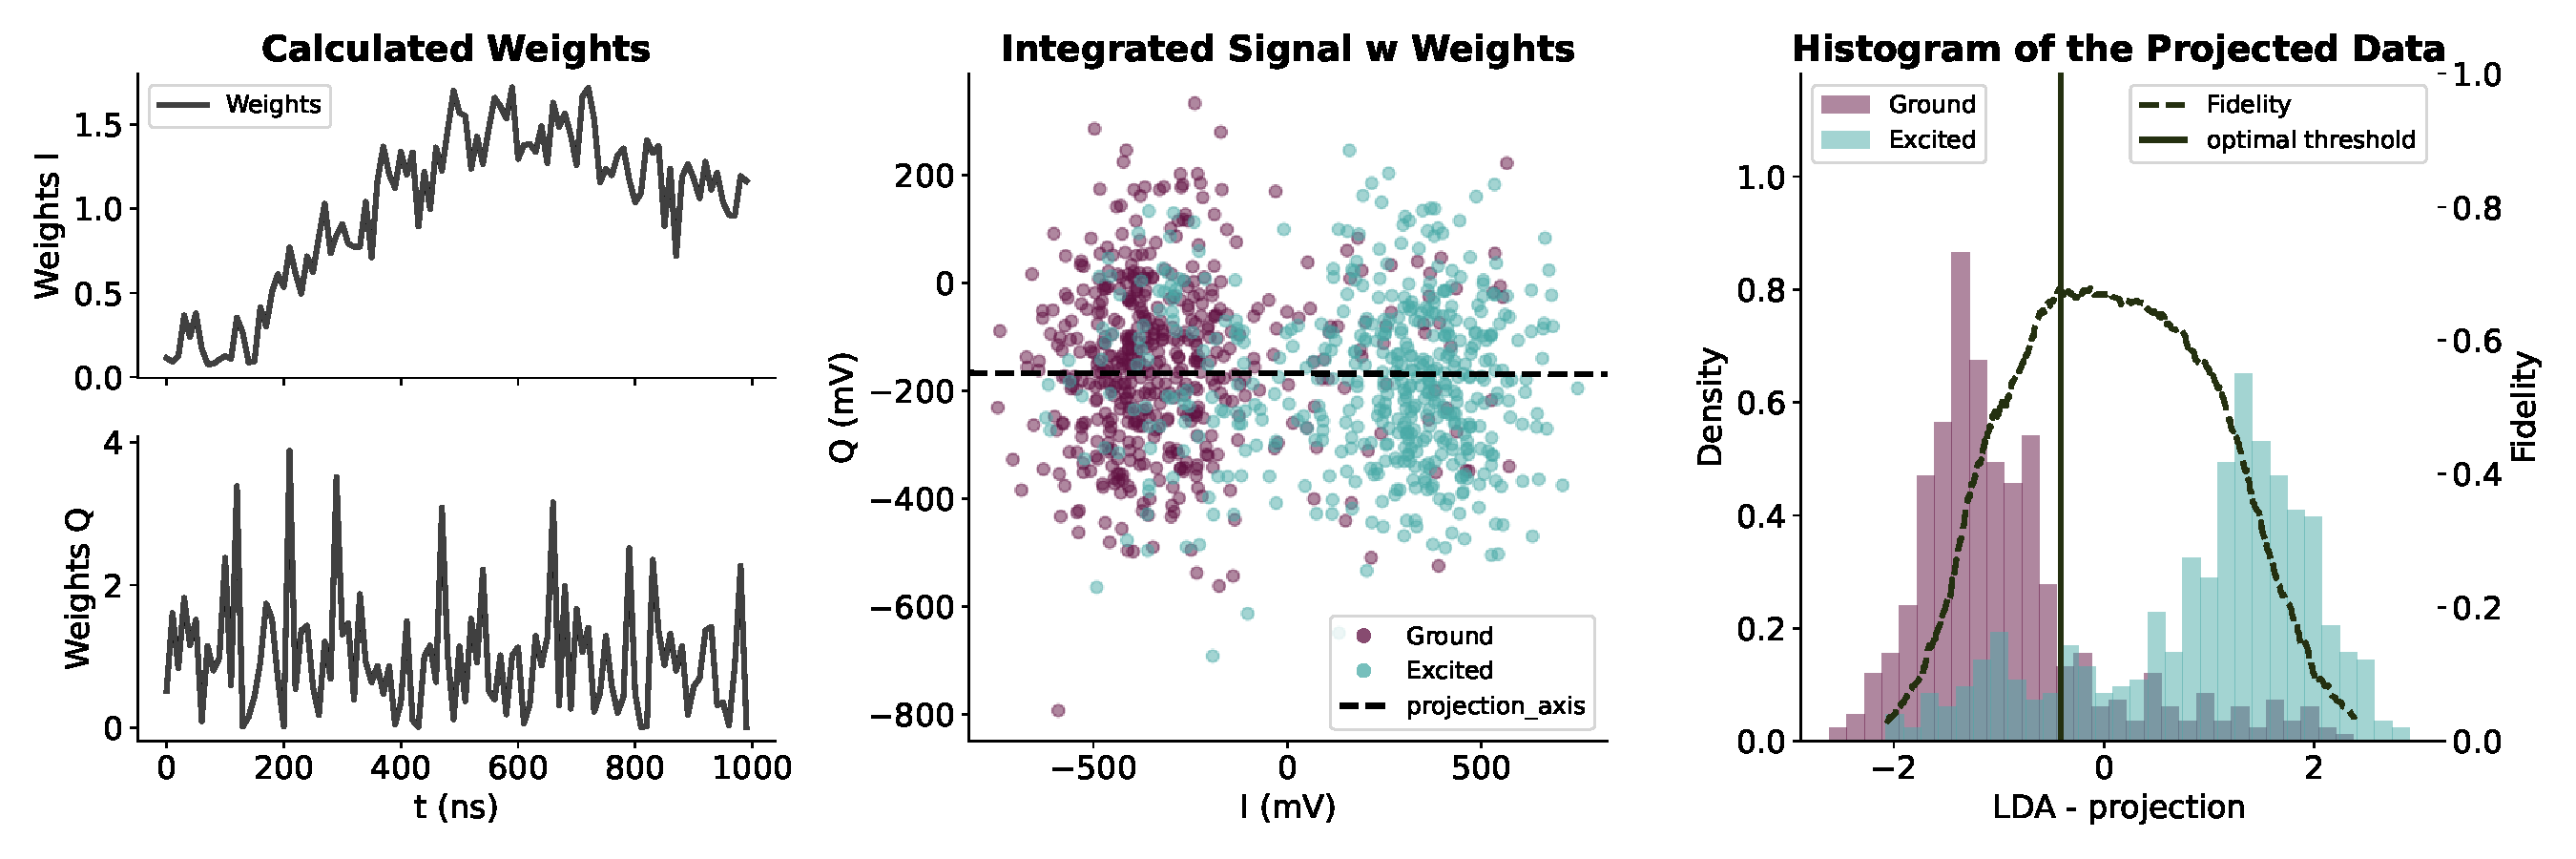
\includegraphics[]{Simulations/readout_simulations/figures/weigted_simulation.pdf}
    \caption{Caption}
    \label{fig:enter-label}
\end{figure*}

